\section{Die Frontend Komponenten}
\label{sec:Frontend}

\subsection{Das Commandline-Tool und seine Erweiterungen}
\subsection{Das Zusammenspiel der Servlets mit dem MCRServlet}
\label{sec:CommonServlets}

Als "ubergeordnetes Servlet mit einigen grundlegenden Funktionalit"aten dient die 
Klasse MCRServlet.
Die Hauptaufgabe von MCRServlet ist dabei die Herstellung der Verbindung zur
Sessionverwaltung (siehe Abschnitt \ref{sec:Sessionverwaltung}).
Das Zusammenspiel der relevanten Klassen ist im folgenden Klassendiagramm 
(Abbildung \ref{fig:MCRServletClasses}) verdeutlicht.

\begin{figure}[h]
  \begin{center}
    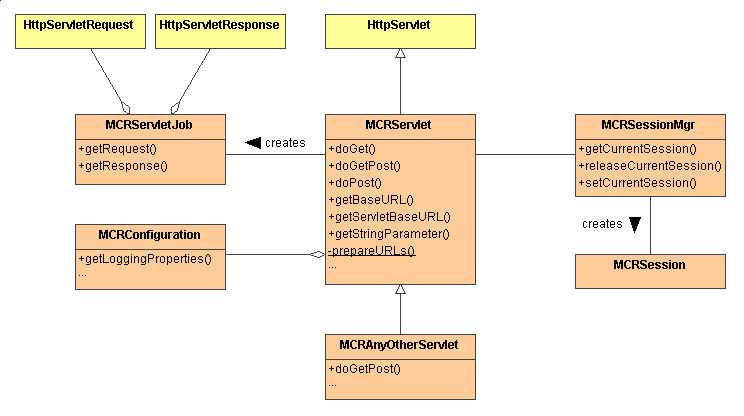
\includegraphics[scale=0.62]{ProgGuide_2Frontend_MCRServlet.jpg}
    \caption{Klassendiagramm Common Servlets}
    \label{fig:MCRServletClasses}
  \end{center}
  \vspace{-1.4cm}
\end{figure} 

Wie an anderen Stellen im MyCoRe-System auch, kann auf Konfigurationsparameter wie
zum Beispiel den Einstellungen f"ur das Logging "uber das statische Attribut
MCRConfiguration zugegriffen werden.
Dies wird ausf"uhrlich in Kapitel \ref{sec:Konfiguration} beschrieben.

MCRServlet selbst ist direkt von HttpServlet abgeleitet.
Sollen andere Servlets im MyCoRe Softwaresystem die von MCRServlet angebotenen 
Funktionen automatisch nutzen, so m"ussen sie von MCRServlet abgeleitet werden.
Im Klassendiagramm ist das durch die stellvertretende Klasse MCRAnyOtherServlet
angedeutet.
Es wird empfohlen, dass die abgeleiteten Servlets die Methoden doGet() und doPost() 
nicht "uberschreiben, denn dadurch werden bei einem eingehenden Request auf jeden 
Fall die Methoden von MCRServlet ausgef"uhrt.

Der Programmablauf innerhalb von MCRServlet ist im folgenden Sequenzdiagramm 
(Abbildung \ref{fig:MCRServletSequenz}) dargestellt.
Bei einem eingehenden Request (doGet() oder doPost()) wird zun"achst an 
MVRServlet.doGetPost() delegiert.
%
\footnote{Bei dieser Delegation wird ein Parameter mitgef"uhrt, "uber den feststellbar 
          ist, ob es sich um einen GET- oder POST-Request gehandelt hat.}

\begin{figure}[h]
  \begin{center}
    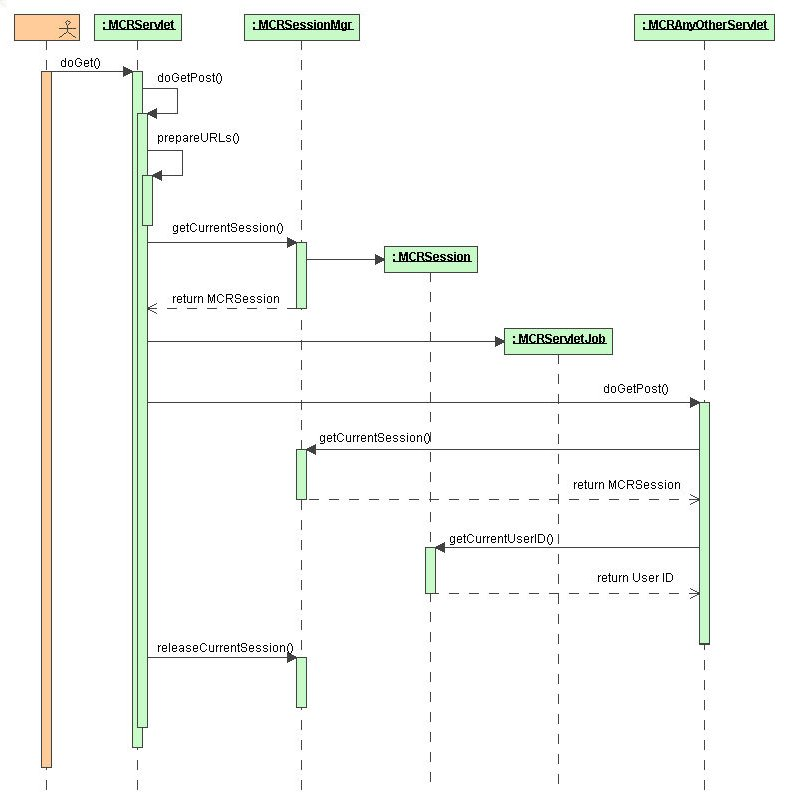
\includegraphics[scale=0.52]{ProgGuide_2Frontend_MCRServletSequenz.jpg}
    \caption{Sequenzdiagramm Common Servlets}
    \label{fig:MCRServletSequenz}
  \end{center}
  \vspace{-1.4cm}
\end{figure} 

Falls nicht schon aus vorhergehenden Anfragen an das MCRServlet bekannt, werden 
in doGetPost() die Base-URL und die Servlet-URL des Systems bestimmt. 
Dabei besteht die Servlet-URL aus der Base-URL und dem angeh"angten String 'servlets/'.
Darauf folgend wird die f�r diese Session zugeh"orige Instanz von MCRSession
bestimmt.
Das Verfahren dazu ist im Ablaufdiagramm \ref{fig:MCRServletFluss} dargestellt. 

\begin{figure}[h]
  \begin{center}
    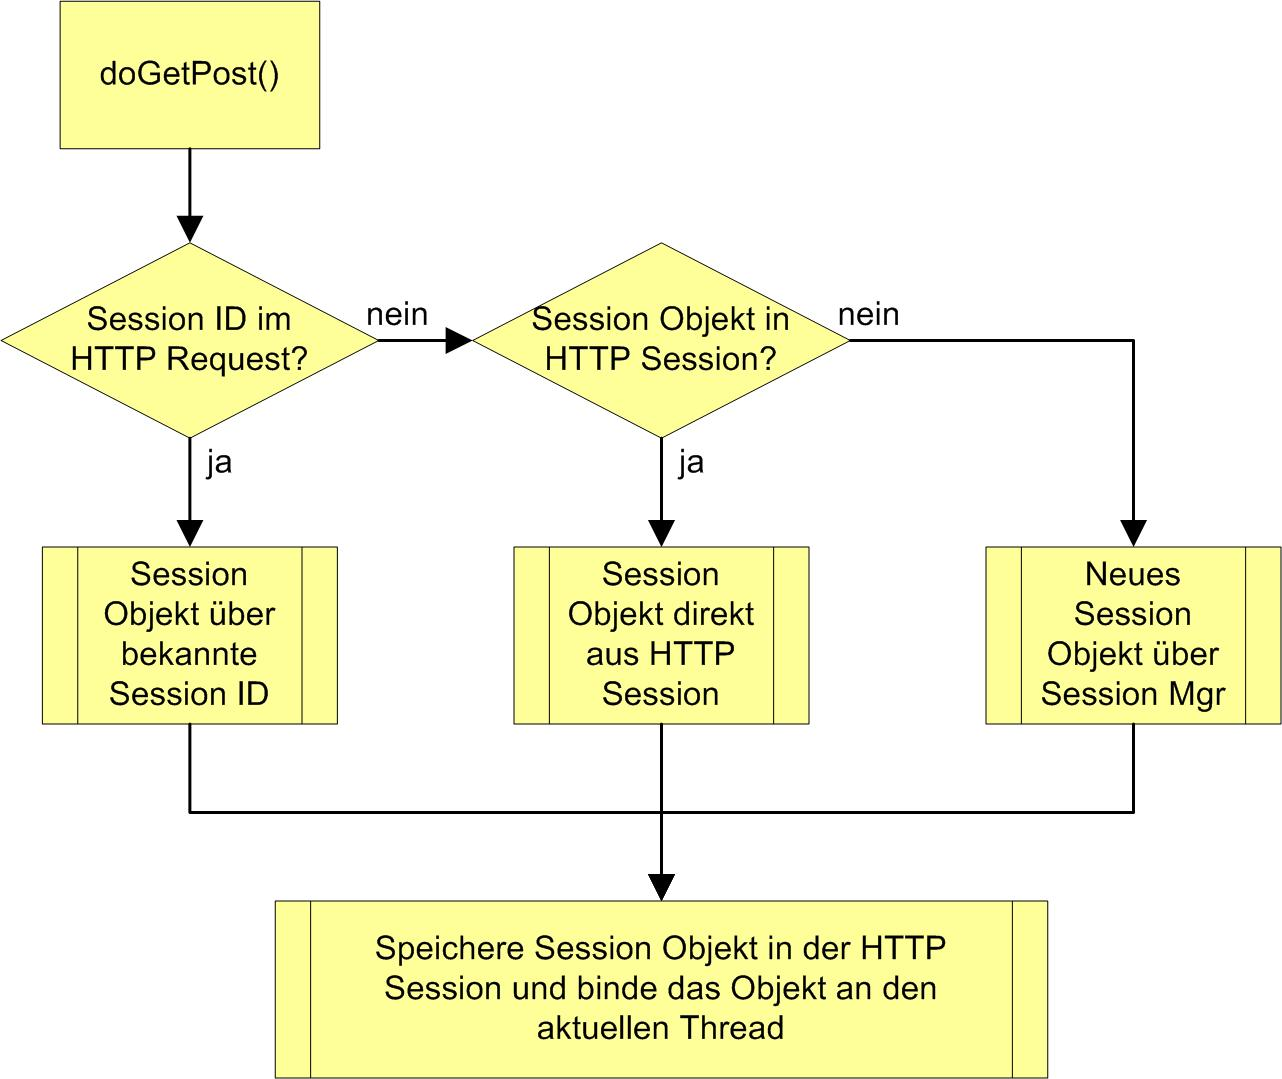
\includegraphics[scale=0.35]{ProgGuide_2Frontend_MCRServletFluss.jpg}
    \caption{Ablaufdiagramm f"ur MCRServlet.doGetPost()}
    \label{fig:MCRServletFluss}
  \end{center}
  \vspace{-1.4cm}
\end{figure} 

Die Session kann bereits durch vorhergehende Anfragen existieren. 
Falls dies der Fall ist, kann das zugeh"orige Session-Objekt entweder "uber eine im 
HttpServletRequest mitgef"uhrte Session ID identifiziert oder direkt der HttpSession
entnommen werden.
Existiert noch keine Session, so wird ein neues Session-Objekt "uber den Aufruf von
MCR\-Session\-Mgr.\-get\-Current\-Session() erzeugt (vergleiche Abschnitt \ref{sec:Sessionverwaltung}).
Nachfolgend wird das Session-Objekt an den aktuellen Thread gebunden und zus"atzlich in der
HttpSession abgelegt.
%
\footnote{Das Speichern des Session-Objekts in der Http-Session ist notwendig, weil in 
          einer typischen Servlet-Engine mit Thread-Pool Umgebung nicht davon ausgegangen 
          werden darf, dass bei aufeinanderfolgenden Anfragen aus demselben Kontext auch 
          derselbe Thread zugeweisen wird. Siehe auch Abschnitt \ref{sec:Sessionverwaltung}.}

Im Sequenzdiagramm \ref{fig:MCRServletSequenz} gehen wir davon aus, dass die Sitzung neu ist
und deswegen ein Session-Objekt "uber MCRSessionMgr.getCurrentSession() erzeugt werden muss.
Schliesslich wird eine Instanz von MCRServletJob erzeugt.
Diese Klasse ist nichts weiter als ein Container f"ur die aktuellen HttpServletRequest- und 
HttpServletResponse Objekte und hat keine weitere Funktionalit"at (siehe Klassendiagramm
\ref{fig:MCRServletClasses}).

An dieser Stelle wird der Programmfluss an das abgeleitete Servlet (in diesem 
Beispiel MCRAnyOtherServlet) delegiert.
Dazu muss das Servlet eine Methode mit der Signatur

{\tt public void doGetPost(MCRServletJob job) \{\}}

implementieren. 
Wie das Sequenzdiagramm \ref{fig:MCRServletSequenz} beispielhaft zeigt, kann 
MCRAnyOtherServlet danach gegebenenfalls auf das Session-Objekt und damit auf die
Kontextinformationen zugreifen.
Der Aufruf an den Session Manager dazu w"are:

{\tt MCRSession mcrSession = MCRSessionMgr.getCurrentSession();}

Es sei bemerkt, dass dies nicht notwendigerweise genau so durchgef"uhrt werden muss.
Da wegen den geschilderten Problemen mit thread-local Variablen in Servlet-Umgebungen
das Session-Objekt auch in der Http-Session abgelegt sein muss, k"onnte man die
Kontextinformationen auch aus der "ubergebenen Instanz von MCRServletJob gewinnen.


\subsection{Das Login-Servlet und MCRSession}

Das Login-Servlet, implementiert durch die Klasse MCRLoginServlet, dient zum 
Anmelden von Benutzern und Benutzerinnen "uber ein Web-Formular.
Die Funktionsweise ist wie folgt:
Wie in Abschnitt \ref{sec:CommonServlets} empfohlen, "uberschreibt MCRLoginServlet 
nicht die von MCRServlet geerbten Standard-Methoden doGet() und doPost().
Meldet sich ein Benutzer oder eine Benutzerin "uber das MCRLoginServlet an, so wird
daher zun"achst die Funktionalit"at von MCRServlet ausgenutzt und die in Abschnitt 
\ref{sec:CommonServlets} beschriebene Verbindung zur Sessionverwaltung herstellt.
Wie dort ebenfalls beschrieben, wird der Programmfluss an das Login-Servlet "uber
die Methode MCRLoginServlet.doGetPost() delegiert.
Der Ablauf in doGetPost() wird im folgenden Diagramm (Abbildung 
\ref{fig:MCRLoginServletFluss}) dargestellt und ist selbsterkl"arend.

\begin{figure}[h]
  \begin{center}
    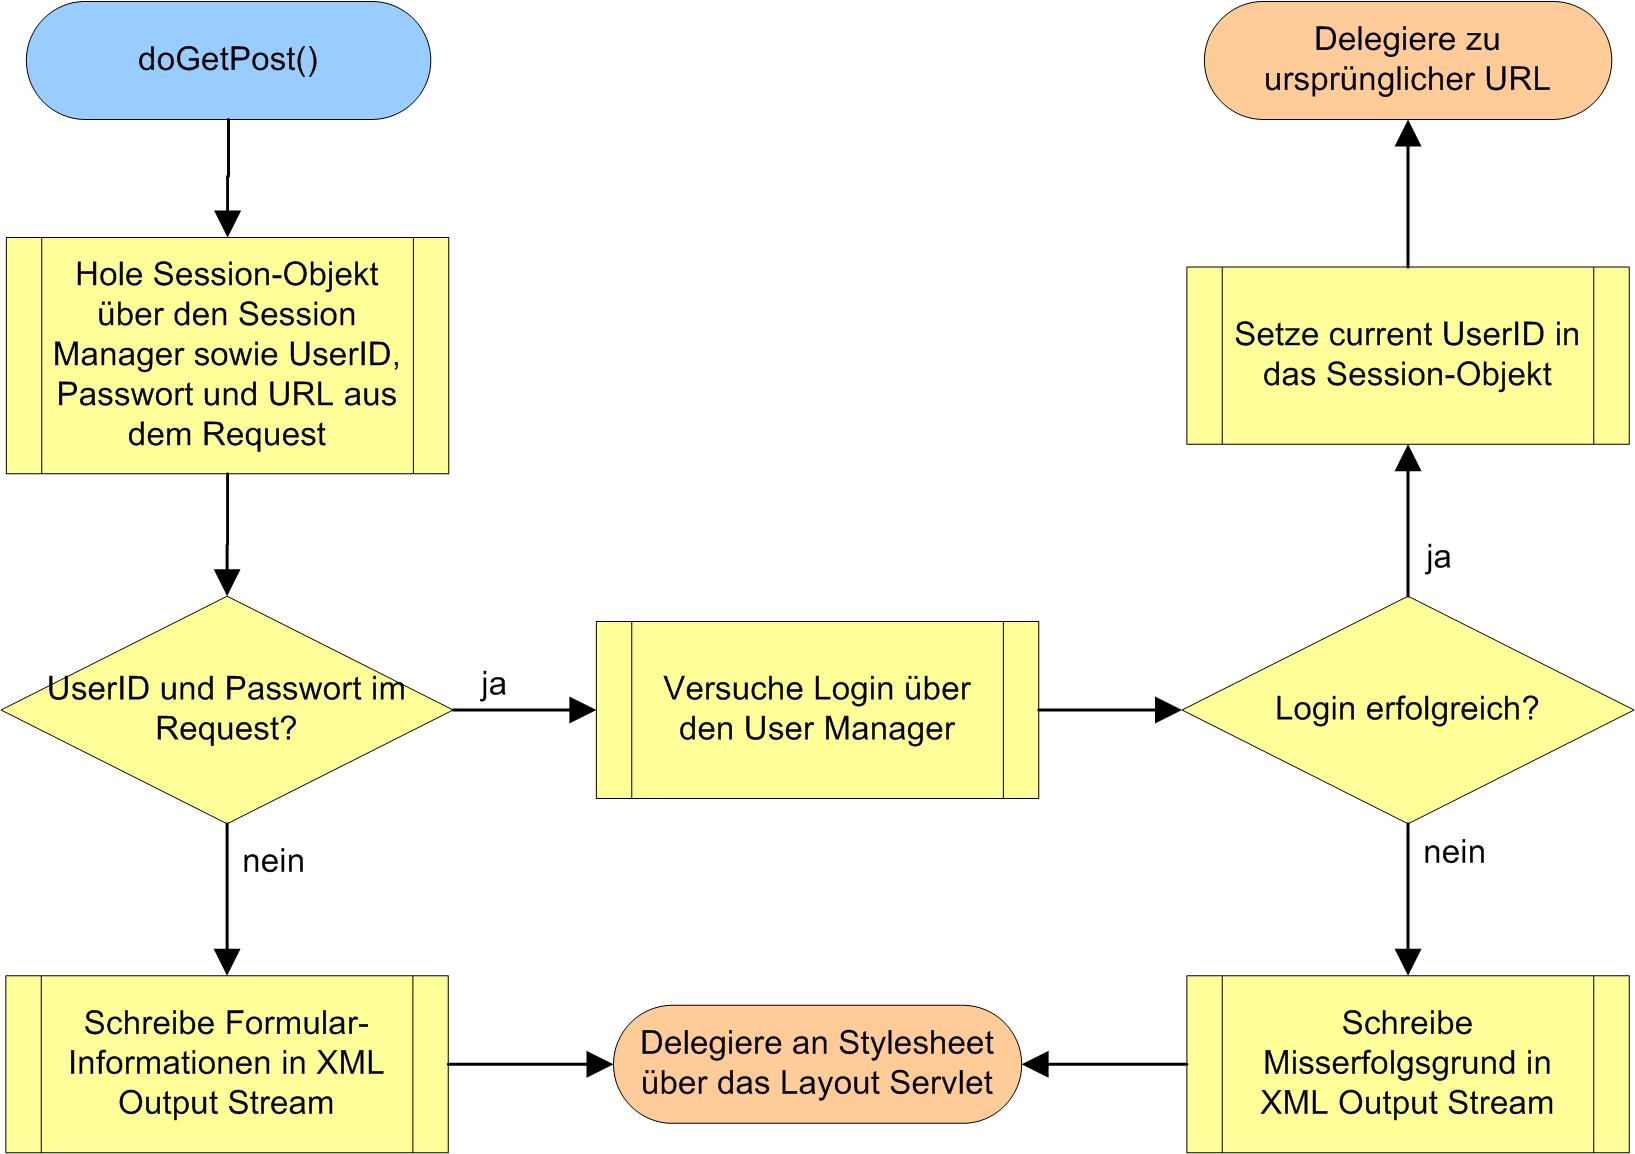
\includegraphics[scale=0.35]{ProgGuide_2Frontend_MCRLoginServletFluss.jpg}
    \caption{Ablaufdiagramm f"ur MCRLoginServlet.doGetPost()}
    \label{fig:MCRLoginServletFluss}
  \end{center}
  \vspace{-1.4cm}
\end{figure} 

Der resultierende XML Output-Stream muss vom zugeh"origen Stylesheet verarbeitet
werden und hat die folgende Syntax:

\vspace{0.5cm}
\lstset{language=XML, fancyvrb=true, frame=btlr, breaklines, prebreak={\space\McrHookSign}}
\begin{lstlisting}[caption={[XML Output des Login Servlets]XML Output des Login Servlets},%
                  captionpos=b, label=lst:XmlLoginServlet, frame=lines]
<mcr_user unknown_user="true|false"
          user_disabled="true|false"
          invalid_password="true|false">
  <guest_id>...</guest_id>
  <guest_pwd>...</guest_pwd>
  <url>...<url>
</mcr_user>
\end{lstlisting}

Bei einer missgl"uckten Anmeldung wird der Grund daf"ur in Form eines Attributes
auf true oder false gesetzt.
Das Stylesheet kann dann die entsprechende Meldung ausgeben.
Die Gast-User ID und das Gast-Passwort werden aus einer Konfigurationsdatei gelesen.
Die URL schlie"slich wird dem Http-Request entnommen und sollte dort von der
aufrufenden Seite bzw. vom aufrufenden Servlet gesetzt sein.
Ist sie nicht gesetzt, so wird die Base-URL des MyCoRe-Systems verwendet.

\subsection{IFS-Servlet}
\subsection{Query-Servlet}
\subsection{Innere Struktur des Editor-Servlets}
\subsection{Innere Struktur des User-Servlets}
